\section{More Results of Improvements in the ME1/1 Local Trigger Algorithm}
\label{app:SLHC_algo_results_more_details}

This chapter presents results of the study of effects of individual improvements described in Sec.~\ref{sec:SLHC_algo_results} on the LCT reconstruction efficiencies.

Three are three baseline configurations of L1 step used in this study:
\begin{itemize}
	\item Baseline 1: SLHC configuration, where the maximum set of improvements is turned off bringing it to 2007 configuration as close as possible. 
	There are only two differences between Baseline 1 and 2007 configurations: separate treatments of ME1a and ME1b, and unganging cathode strips in ME1a;
	\item Baseline 2: Baseline 1 configuration with all improvements on the ALCT and CLCT processors level turned on;
	\item SLHC configuration itself.
\end{itemize}

Improvements on the level of TMB are related to the following configuration parameters (see Sec.~\ref{sec:common_conf}):
\begin{itemize}
	\item matchTrigWindowSize: 7BX to 3BX;
	\item alctUseCorrectedBx: False to True
	\item clctUseCorrectedBx: False to True;
	\item clctToAlct: True to False;
	\item tmbDropUsedClcts and matchEarliestClctME11Only: True to False;
	\item tmbCrossBxAlgorithm: 0 to 1;
	\item tmbReadoutEarliest2: True to False;
\end{itemize}

\newpage

\begin{figure} [h!]
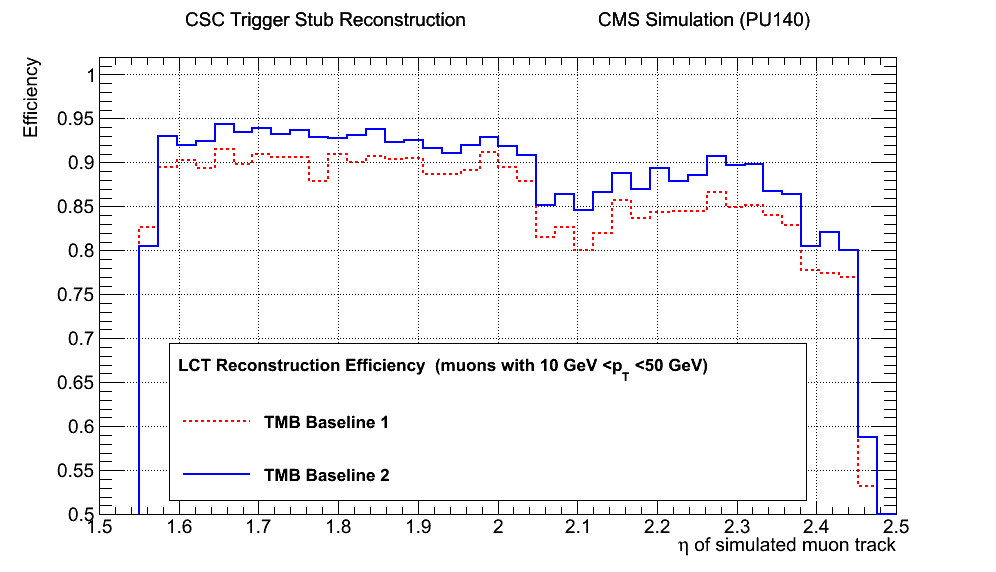
\includegraphics[width=0.98\textwidth]{figures/PU140_Improv_from1_to_2.png}
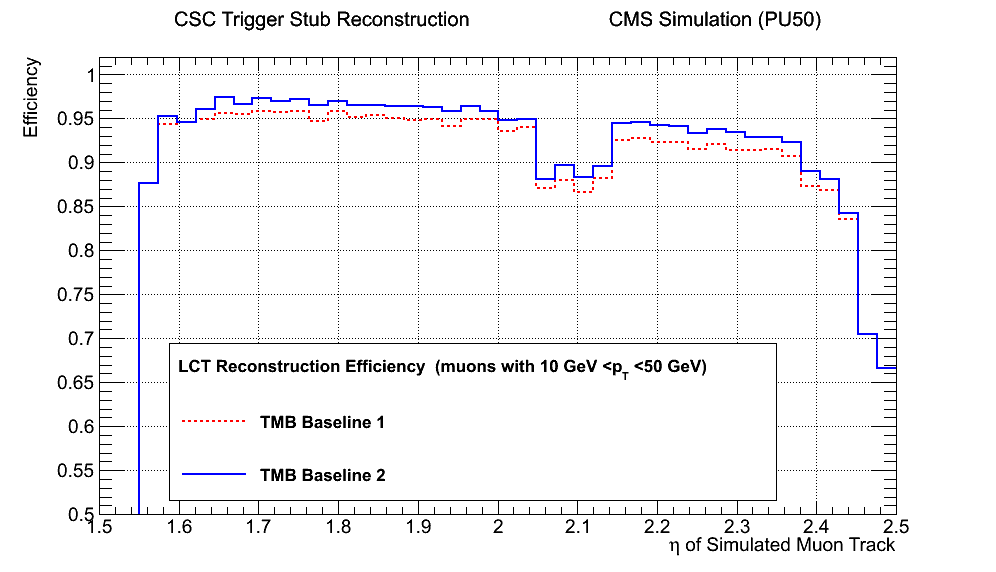
\includegraphics[width=0.98\textwidth]{figures/PU50_Improv_from1_to_2.png}
\caption{LCT reconstruction efficiency in ME1/1 station for PU140 (top) and PU50 (bottom). The efficiencies increase due to change from TMB Baseline 1 configuration to TMB Baseline 2 configuration. Muons with transverse momentum $10$~GeV$<p_T<50$~ GeV are used in the analysis.}
\label{fig:From1to2}
\end{figure}
\begin{figure} [h!]
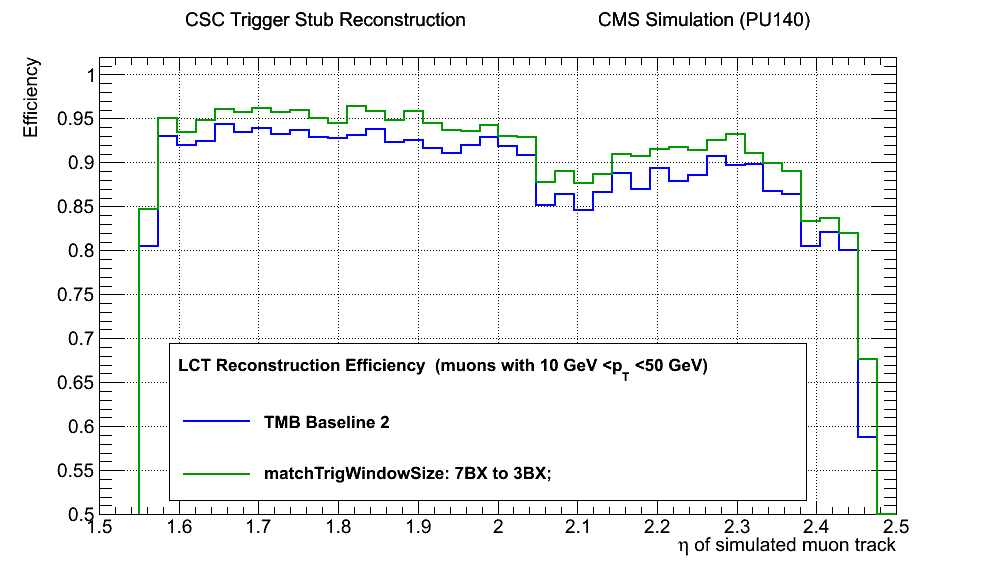
\includegraphics[width=0.98\textwidth]{figures/PU140_Improv_from2_to_3.png}
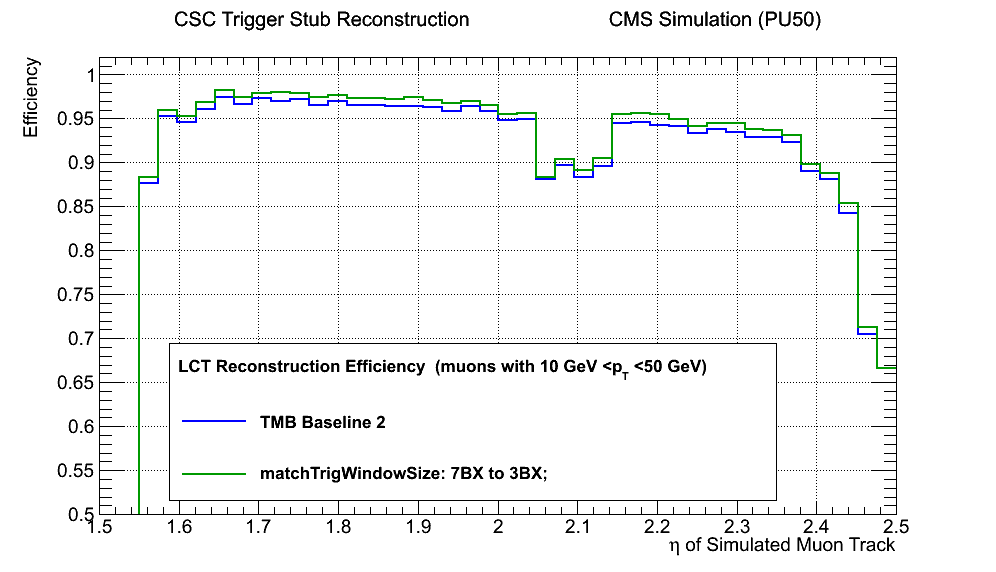
\includegraphics[width=0.98\textwidth]{figures/PU50_Improv_from2_to_3.png}
\caption{LCT reconstruction efficiency in ME1/1 station for PU140 (top) and PU50 (bottom). The efficiencies increase due to change of \textcolor{blue}{matchTrigWindowSize} from 7BX to 3BX. Muons with transverse momentum $10$~GeV$<p_T<50$~ GeV are used in the analysis.}
\label{fig:From2to3}
\end{figure}
\begin{figure} [h!]
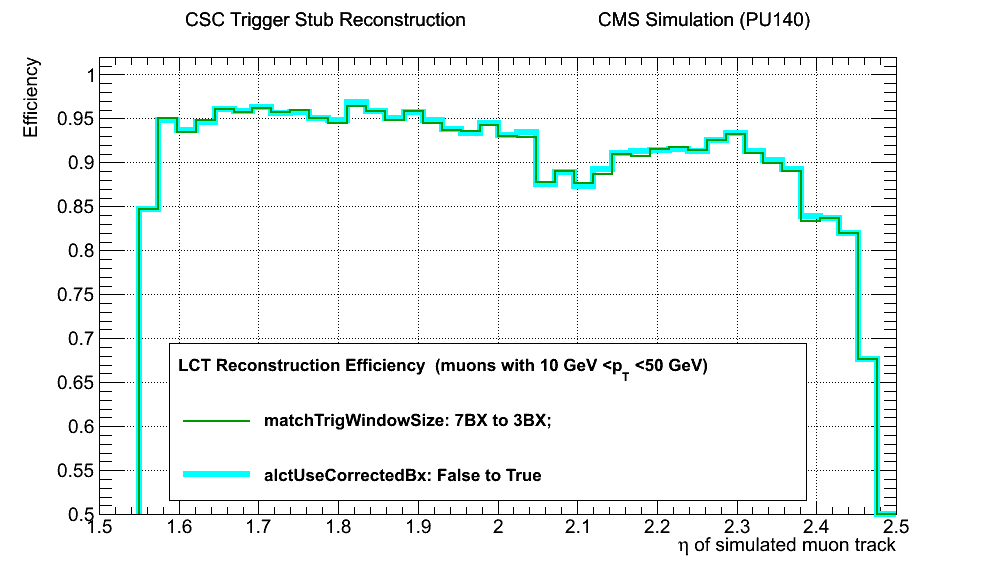
\includegraphics[width=0.98\textwidth]{figures/PU140_Improv_from3_to_4.png}
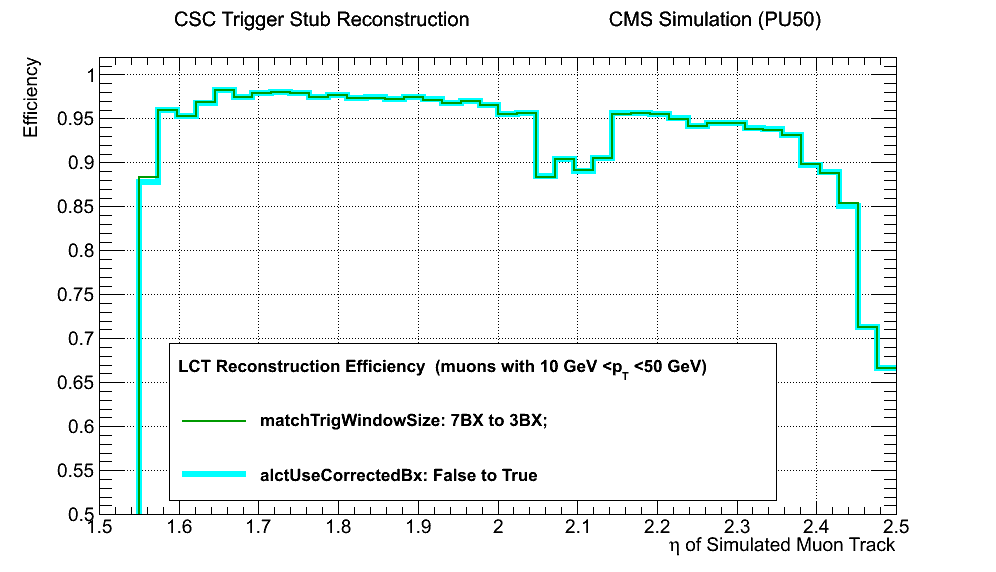
\includegraphics[width=0.98\textwidth]{figures/PU50_Improv_from3_to_4.png}
\caption{LCT reconstruction efficiency in ME1/1 station for PU140 (top) and PU50 (bottom). The efficiencies increase due to change of \textcolor{blue}{alctUseCorrectedBx} from False to True. Muons with transverse momentum $10$~GeV$<p_T<50$~ GeV are used in the analysis.}
\label{fig:From3to4}
\end{figure}
\begin{figure}[h!]
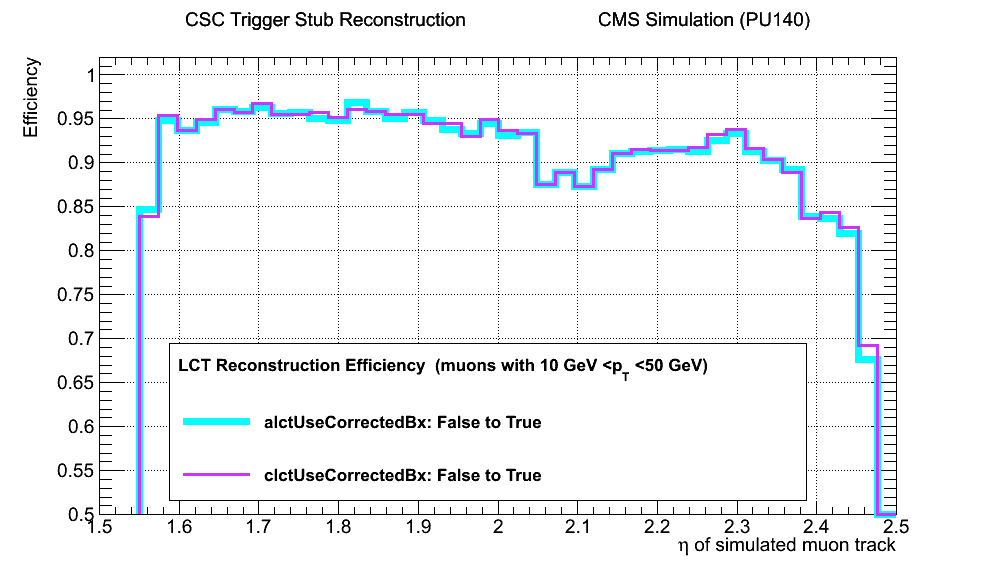
\includegraphics[width=0.98\textwidth]{figures/PU140_Improv_from4_to_5.png}
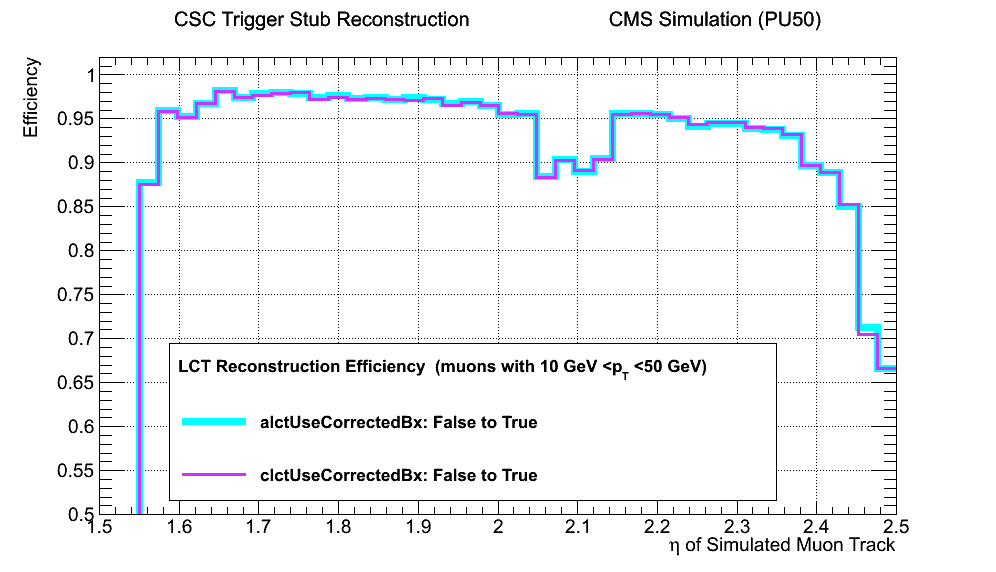
\includegraphics[width=0.98\textwidth]{figures/PU50_Improv_from4_to_5.png}
\caption{LCT reconstruction efficiency in ME1/1 station for PU140 (top) and PU50 (bottom). The efficiencies increase due to change of \textcolor{blue}{clctUseCorrectedBx} from False to True. Muons with transverse momentum $10$~GeV$<p_T<50$~ GeV are used in the analysis.}
\label{fig:From4to5}
\end{figure}
\begin{figure}[h!]
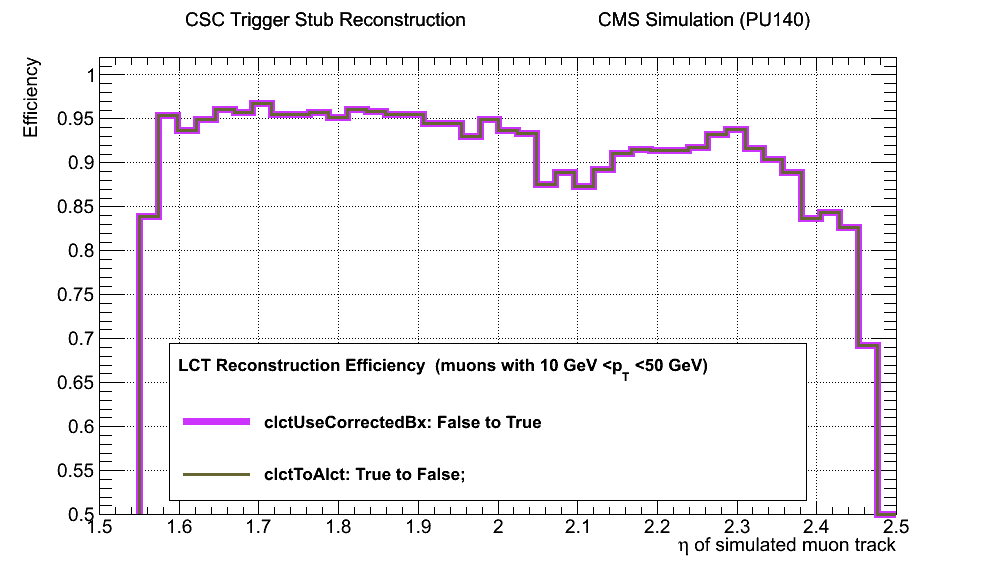
\includegraphics[width=0.98\textwidth]{figures/PU140_Improv_from5_to_6.png}
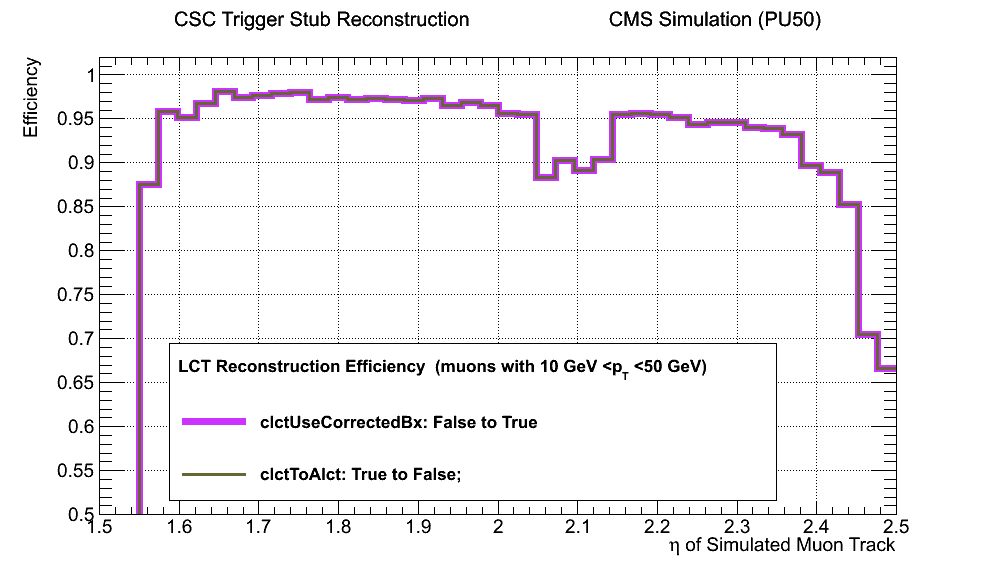
\includegraphics[width=0.98\textwidth]{figures/PU50_Improv_from5_to_6.png}
\caption{LCT reconstruction efficiency in ME1/1 station for PU140 (top) and PU50 (bottom). The efficiencies increase due to change of \textcolor{blue}{clctToAlct} from True to False. Muons with transverse momentum $10$~GeV$<p_T<50$~ GeV are used in the analysis.}
\label{fig:From5to6}
\end{figure}
\begin{figure}[h!]
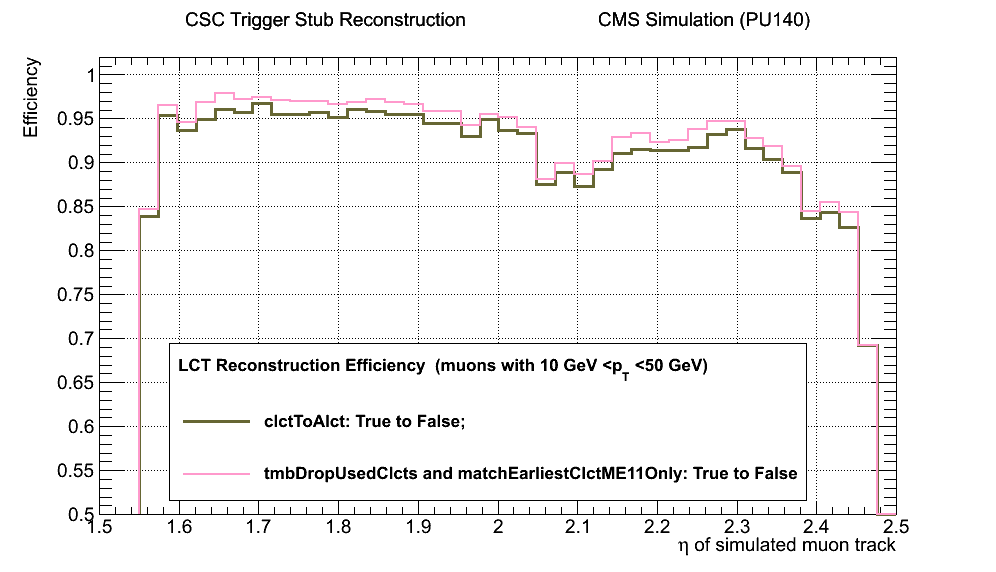
\includegraphics[width=0.98\textwidth]{figures/PU140_Improv_from6_to_7.png}
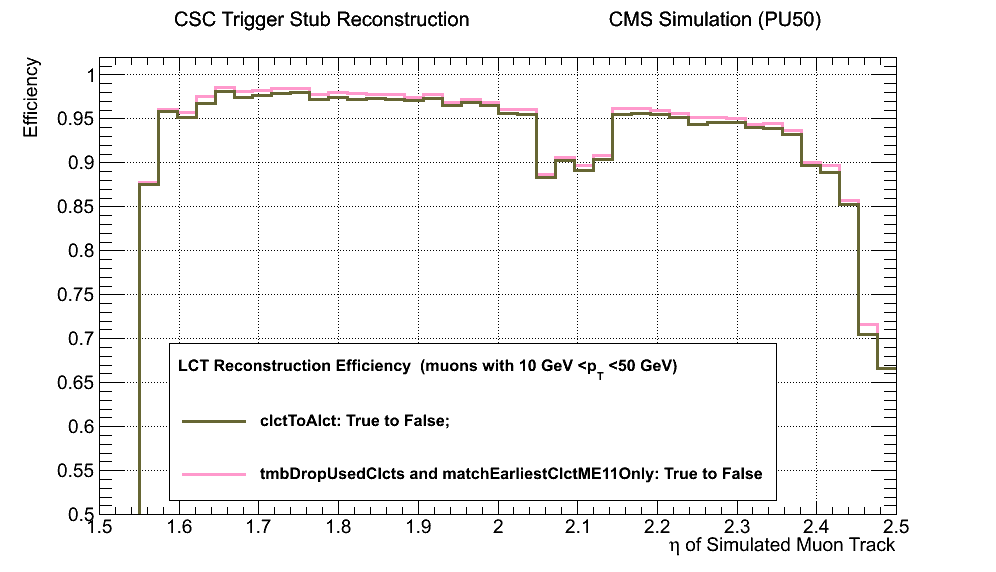
\includegraphics[width=0.98\textwidth]{figures/PU50_Improv_from6_to_7.png}
\caption{LCT reconstruction efficiency in ME1/1 station for PU140 (top) and PU50 (bottom). The efficiencies increase due to change of \textcolor{blue}{tmbDropUsedClcts} and \textcolor{blue}{matchEarliestClctME11Only} from True to False. Muons with transverse momentum $10$~GeV$<p_T<50$~ GeV are used in the analysis.}
\label{fig:From6to7}
\end{figure}
\begin{figure}[h!]
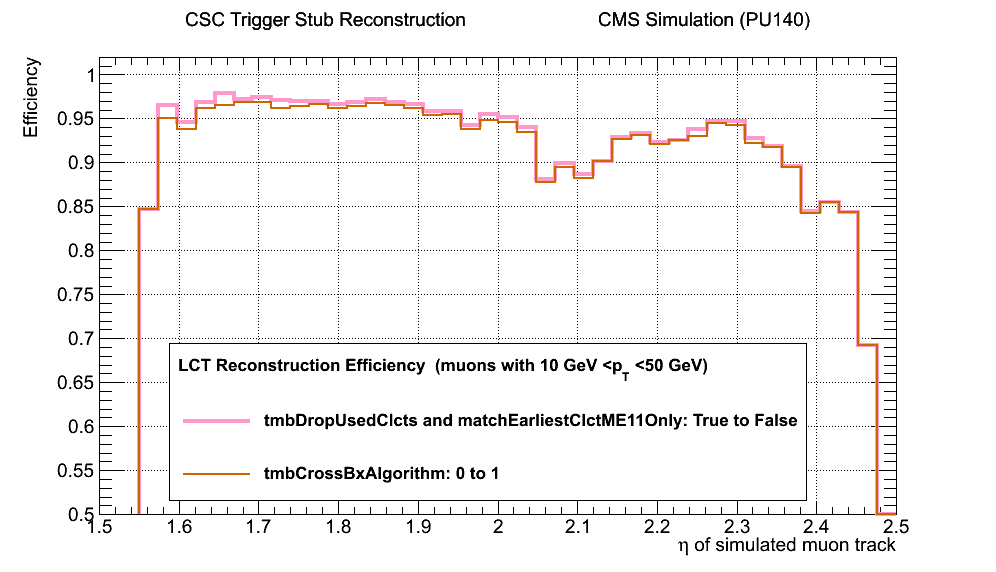
\includegraphics[width=0.98\textwidth]{figures/PU140_Improv_from7_to_8.png}
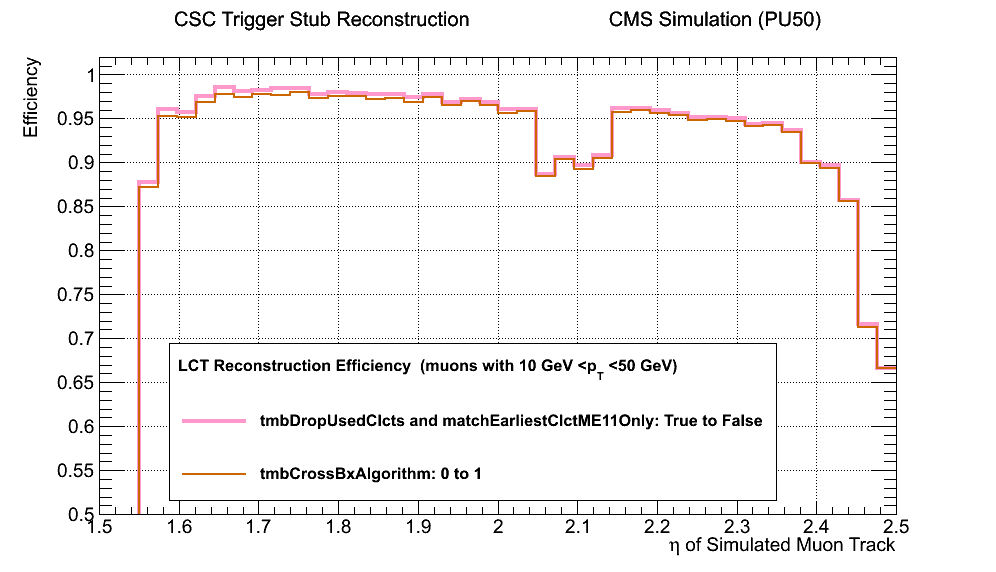
\includegraphics[width=0.98\textwidth]{figures/PU50_Improv_from7_to_8.png}
\caption{LCT reconstruction efficiency in ME1/1 station for PU140 (top) and PU50 (bottom). The efficiencies increase due to change of \textcolor{blue}{tmbCrossBxAlgorithm} from 0 to 1. Muons with transverse momentum $10$~GeV$<p_T<50$~ GeV are used in the analysis.}
\label{fig:From7to8}
\end{figure}
\begin{figure}[h!]
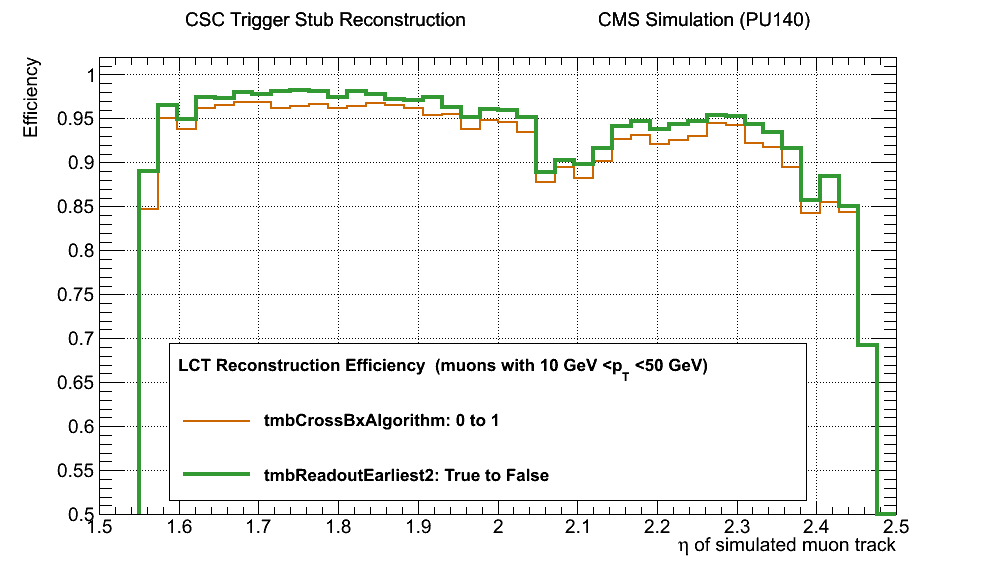
\includegraphics[width=0.98\textwidth]{figures/PU140_Improv_from8_to_9.png}
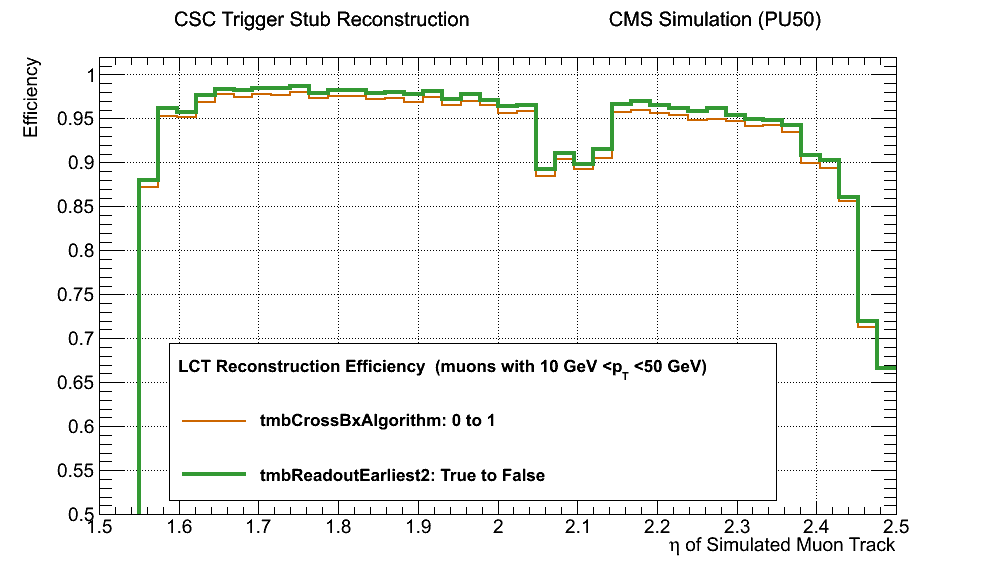
\includegraphics[width=0.98\textwidth]{figures/PU50_Improv_from8_to_9.png}
\caption{LCT reconstruction efficiency in ME1/1 station for PU140 (top) and PU50 (bottom). The efficiencies increase due to change of \textcolor{blue}{tmbReadoutEarliest2} from True to False. Muons with transverse momentum $10$~GeV$<p_T<50$~ GeV are used in the analysis.}
\label{fig:From8to9}
\end{figure}
\begin{figure}[h!]
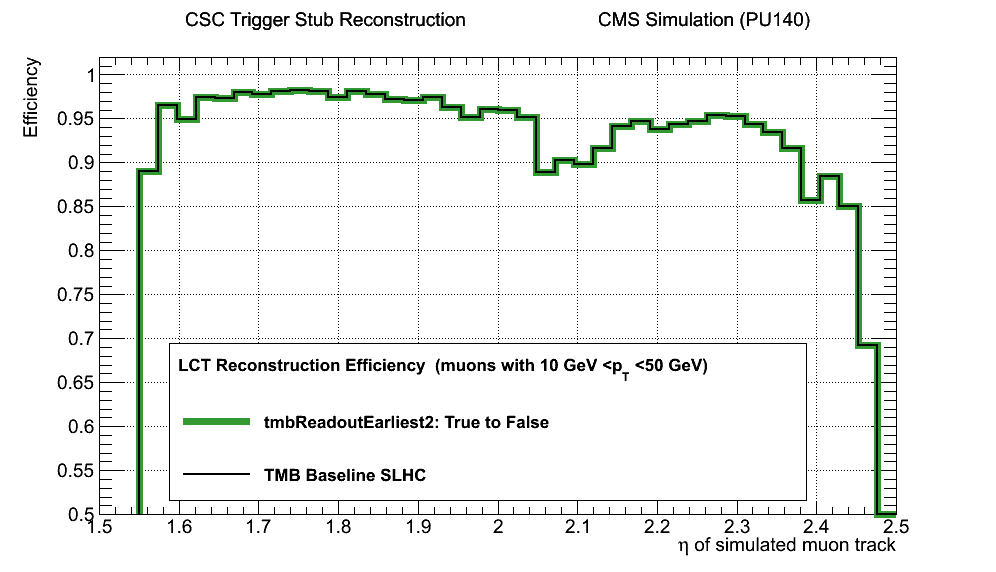
\includegraphics[width=0.98\textwidth]{figures/PU140_Improv_from9_to_10.png}
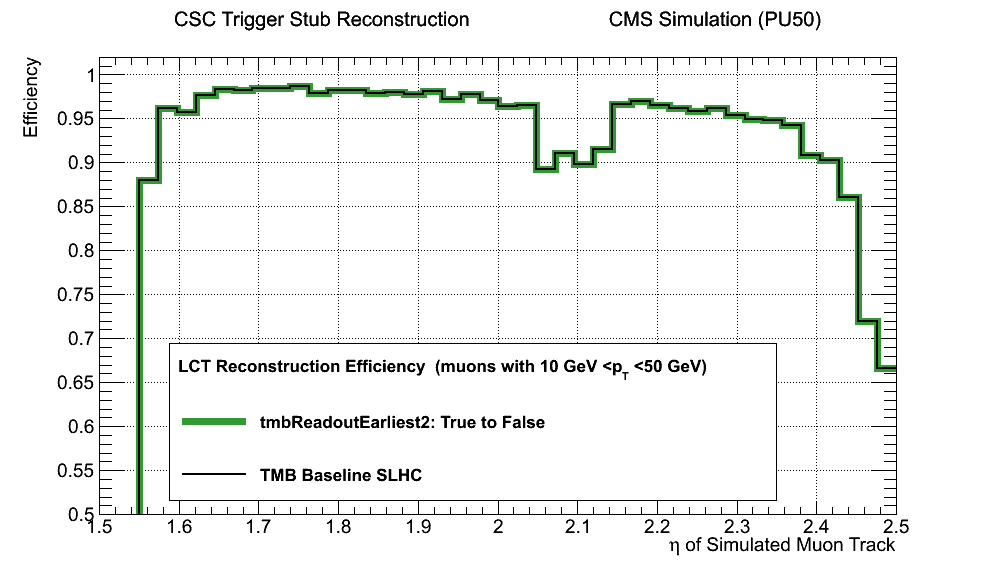
\includegraphics[width=0.98\textwidth]{figures/PU50_Improv_from9_to_10.png}
\caption{LCT reconstruction efficiency in ME1/1 station for PU140 (top) and PU50 (bottom). After the last improvment we are on the current TMB SLHC suggested configuration therefore it's expected that the efficiencies agree. Muons with transverse momentum $10$~GeV$<p_T<50$~ GeV are used in the analysis.}
\label{fig:From9to10}
\end{figure}